\documentclass[11pt]{article}

\usepackage{amssymb,amsmath}
\usepackage{times,psfrag,epsf,epsfig,graphics,graphicx,caption}
\usepackage{enumitem}
\usepackage{algorithm}
\usepackage{algorithmic}

\begin{document}
\date{}

\title{PHSX 343: Assignment 3}

\author{William Jardee}

\maketitle


\section*{Problem 1}

\begin{enumerate}[label=\alph*)]
  \item 
  \parbox{}{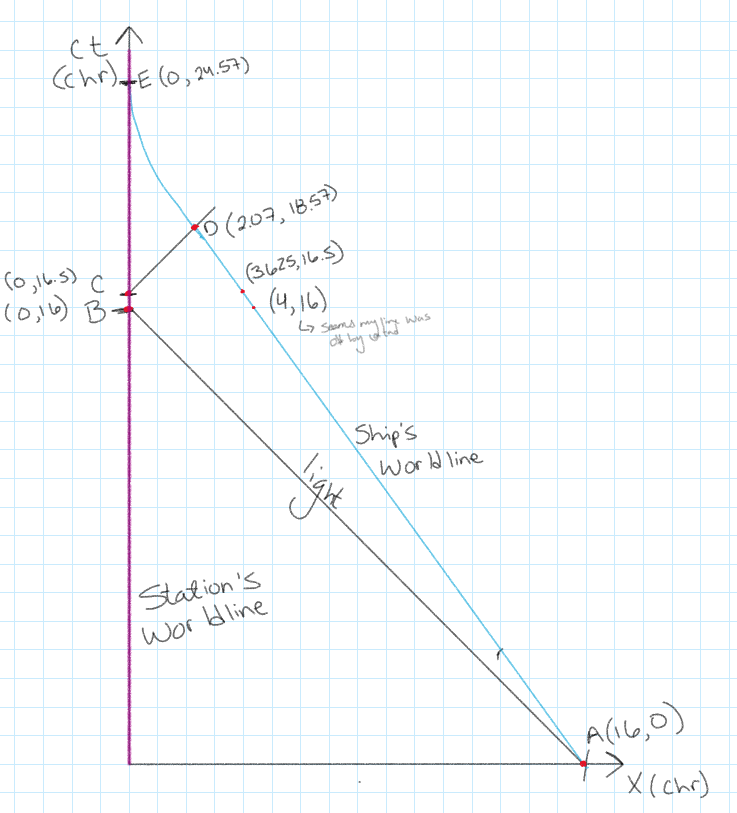
\includegraphics[width = 300 pt]{Homework3/homework 3.PNG}}\\
  
 To help get the location of the ship let's write the line it follows. Through simple geometry we get $ct=-\frac{4}{3}x+\frac{64}{3}$. Since light always travels with a slope of 1, event B will arrive at $ct = 16$. Event C happens half an hour later, at $t = 16.5$. Using a new line for the light leaving C, $ct = x+16.5$, the intercept becomes $x=2.07$, $ct = 18.6$. We can do our best to draw a quadratic deceleration to $ct = 24.6$ as the ship comes in to land. 
 
\item
\[x = x_0 +vt+\frac{1}{2}at^2 \rightarrow -2.07 (c*hr) = -0.750c(6hr) +\frac{1}{2}a(6hr)^2\]\\
 \[-2.07 = -0.750(6)+\frac{1}{2}a(36hr)\left(3600\frac{s}{hr}\right)\left( \frac{1}{c}\right) \]\\
 \[\frac{2c*(-2.07+0.75(6))}{(36)(3600)} = a \left[\frac{m}{s^2}\right]\]\\
 \[a \approx 1.12x10^4 \frac{m}{s^2} \approx 1.15x10^3 g\]
\end{enumerate}

\section*{Problem 2}
\begin{enumerate}[label=\alph*)]
    \item 
    
    \parbox{}{ 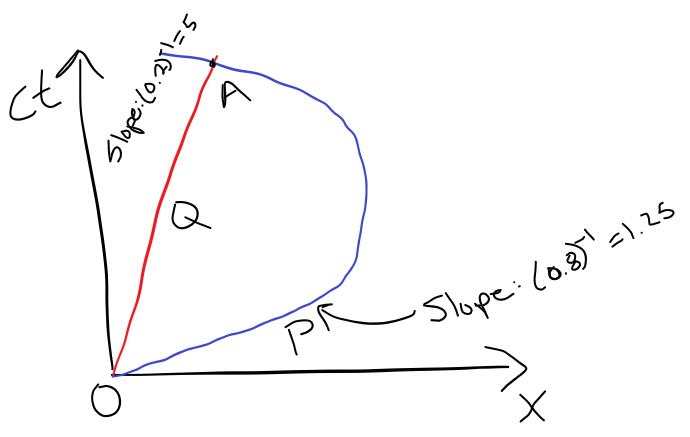
\includegraphics[width = 200 pt]{Homework3/homework 3.1.PNG}}
    
\item
The two clocks will not necessarily read the same time as all our rules pertain to inertial frames, but the P frame is accelerating back towards $x=0$, so it is not inertial.

\item
\begin{itemize}
    \item Coordinate Time:\\
        O and A define a coordinate time as they are both inertial and one at each event\\
        Q is also defines a coordinate time as it is present at each event and traveling at a constant speed.\\
        P does not define a coordinate time as it is not an inertial frame
    \item Proper Time:\\
        O and A do not define a proper time as they are different clocks at different events\\
        Q and P each independently define proper time as they are each at the event and are one clock. The definition does not include needing to be inertial.
    \item $\Delta  /c$:\\
        Q is the only clock that defines $\frac{1}{c}$ time as it is the only clock that is at both events and is inertial.
\end{itemize}
\end{enumerate}

\section*{Problem 3}
    \parbox{}{ 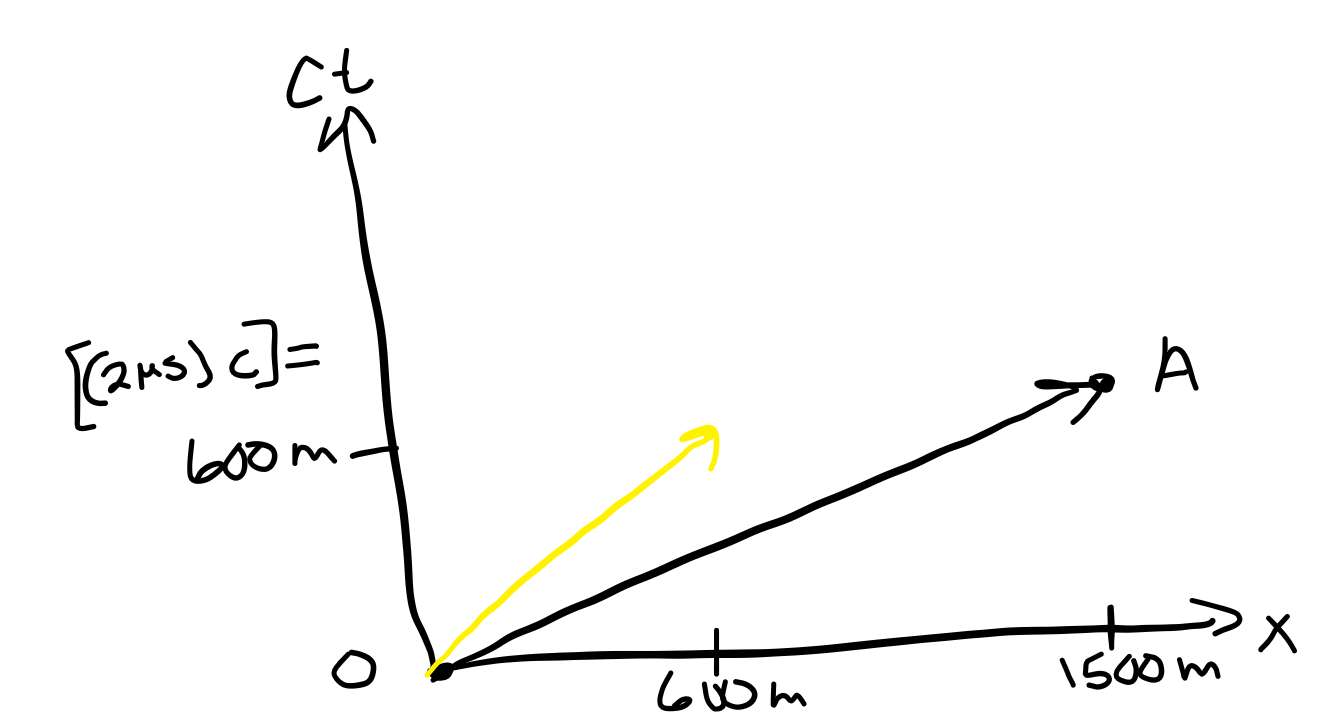
\includegraphics[width = 200 pt]{Homework3/homework 3.2.PNG}}\\\\
    \[v = \frac{1500m}{2.00x10^{-6}*c} = 2.5c\]
    To be at both the origin and event A, something would have to travel 2.5 times the speed of light, so a light pulse could not travel between the two.



\end{document}
